\subsection{Opdracht 05}

Vermoedelijk zijn niet alle Film ID�s in gebruik. Geef het statement dat de langste aaneengesloten reeks geeft van Film ID�s in jouw database.

\subsubsection{Versie 01}

TODO: Marc

\lstinputlisting[language=SQL]{sql/marc/opdracht-05a.sql}
\begin{figure}
    \centering
    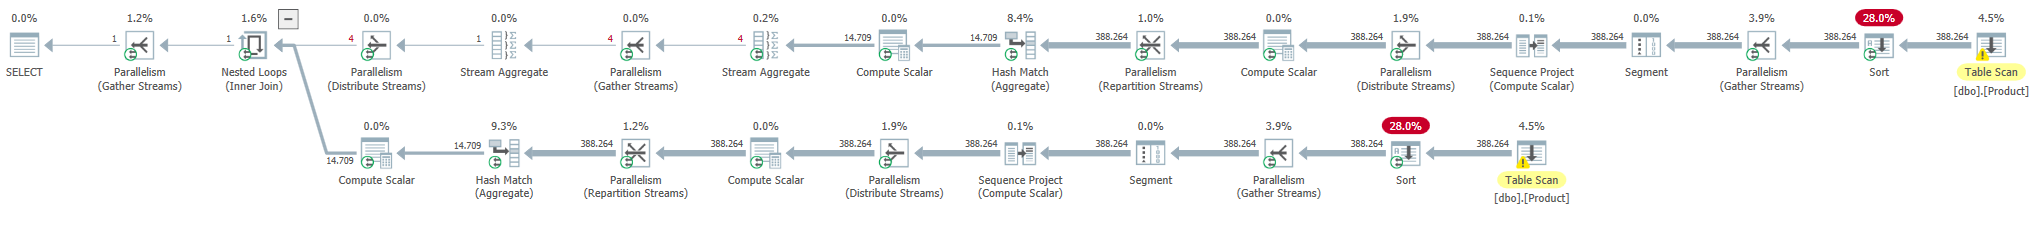
\includegraphics[width=1\textwidth]{image/marc/opdracht-05a.PNG}
    \caption{Queryplan Opdracht 05 Versie 01}
\end{figure}

\subsubsection{Versie 02}

TODO: Joey

\lstinputlisting[language=SQL]{sql/joey/opdracht-05a.sql}
\begin{figure}
    \centering
    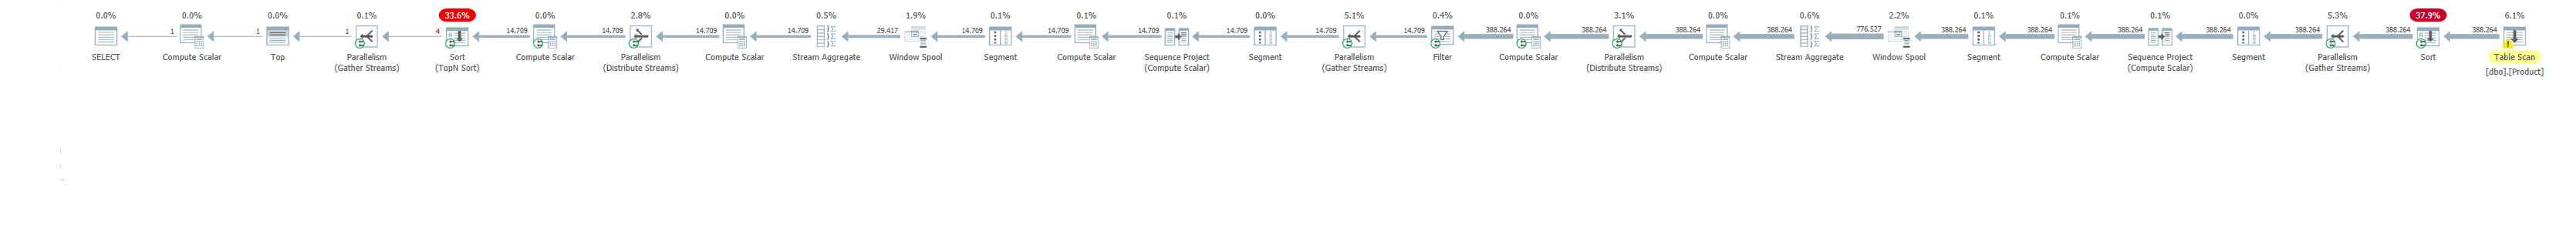
\includegraphics[width=1\textwidth]{image/joey/opdracht-05a.PNG}
    \caption{Queryplan Opdracht 05 Versie 02}
\end{figure}


\subsubsection{Versie 03}

In de eerste CTE worden de rijnummers, en de product\_id weergegven. Als 3e kolom word het verschil tussen deze 2 weergegeven.
Wanneer deze diff verschilt van de vorige diff waarde weet je dat er een gap is.
In de tweede CTE word er eerst gegroepeerd op de diff waarde. Nu hebben we alle islands gegroepeerd.
Vervolgens pakken we de hoogste en laagste waarde van een island, en berekenen we de lengte.
Als laatste stap halen we de hoogste waarde voor lengte er uit, en presenteren we die.

\lstinputlisting[language=SQL]{sql/nick/opdracht-05a.sql}
\begin{figure}
    \centering
    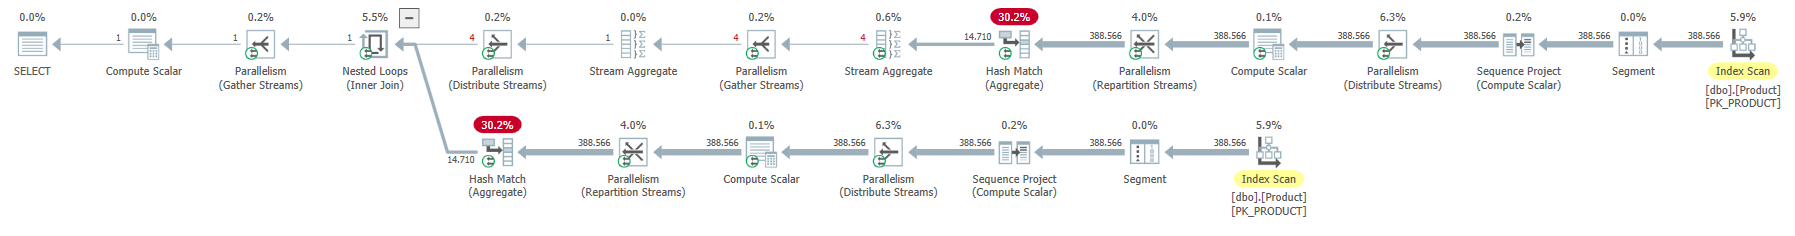
\includegraphics[width=1\textwidth]{image/nick/opdracht-05a.PNG}
    \caption{Queryplan Opdracht 05 Versie 02}
\end{figure}


\subsubsection{Conclusie}

\begin{tabular}{ || l | l | l | l | l | l | l | l | l | l | l | l | 1 | 1 | l | 1 | 1 || }
    \hline
    \textbf{Statement} & \textbf{Est Cost \%} & \textbf{Compile Time} & \textbf{Duration} & \textbf{CPU} & \textbf{Est CPU Cost \%} & \textbf{Est IO Cost \%} \\
    \hline
    \hline
    Versie01  & 36,1\%  & 8  & 1.908  & 2.401  & 36,7\% & 29,1\% \\
    \hline
    Versie02  & 48.8\%  & 18  & 1.779  & 3.207  & 48,3\% & 55,4\%  \\
    \hline
    Versie03  & 15,0\%  & 10  & 1.252  & 2.104  & 15,0\% & 15,5\%  \\
    \hline
\end{tabular}
\newline
\newline
\begin{tabular}{ || l | l | l | l | l | l | l | l | l | l | l | l | 1 | 1 | l | 1 | 1 || }
    \hline
    \textbf{Statement} &  \textbf{Est Rows} & \textbf{Actual Rows} & \textbf{RID Lookups} & \textbf{Parallel} & \textbf{Sort} & \textbf{Table Scan} & \textbf{Hash Match} \\
    \hline
    \hline
    Versie01  & 1        & 1  & 0  & 11  & 2  & 1  & 0 \\
    \hline
    Versie02  & 388.403  & 1  & 0  & 21  & 2  & 2  & 2 \\
    \hline
    Versie03  & 1        & 1  & 0  & 13  & 0  & 0  & 2 \\
    \hline
\end{tabular}

\paragraph{
Hier komt dus een lang verhaal over welke query het beste is, en waarom
}
